% Created 2025-02-10 Mon 13:52
% Intended LaTeX compiler: pdflatex
\documentclass[11pt]{article}
\usepackage[utf8]{inputenc}
\usepackage[T1]{fontenc}
\usepackage{graphicx}
\usepackage{longtable}
\usepackage{wrapfig}
\usepackage{rotating}
\usepackage[normalem]{ulem}
\usepackage{amsmath}
\usepackage{amssymb}
\usepackage{capt-of}
\usepackage{hyperref}
\date{}
\title{Modernising Earthquake Simulation Workflows}
\hypersetup{
 pdfauthor={},
 pdftitle={Modernising Earthquake Simulation Workflows},
 pdfkeywords={},
 pdfsubject={},
 pdfcreator={Emacs 30.0.93 (Org mode 9.7.19)}, 
 pdflang={English}}
\begin{document}

\maketitle
\section*{Context}
\label{sec:orga56ed24}

\subsection*{What We Do}
\label{sec:orgc4636dc}
\begin{itemize}
\item Support earthquake researchers at UC Civil and Natural Resources Engineering department.
\item Primary focus: Ground motion simulation software.
\end{itemize}
\subsection*{Cybershake New Zealand}
\label{sec:org06d9fab}
\subsection*{Researcher Outputs}
\label{sec:orgb654618}
\begin{center}
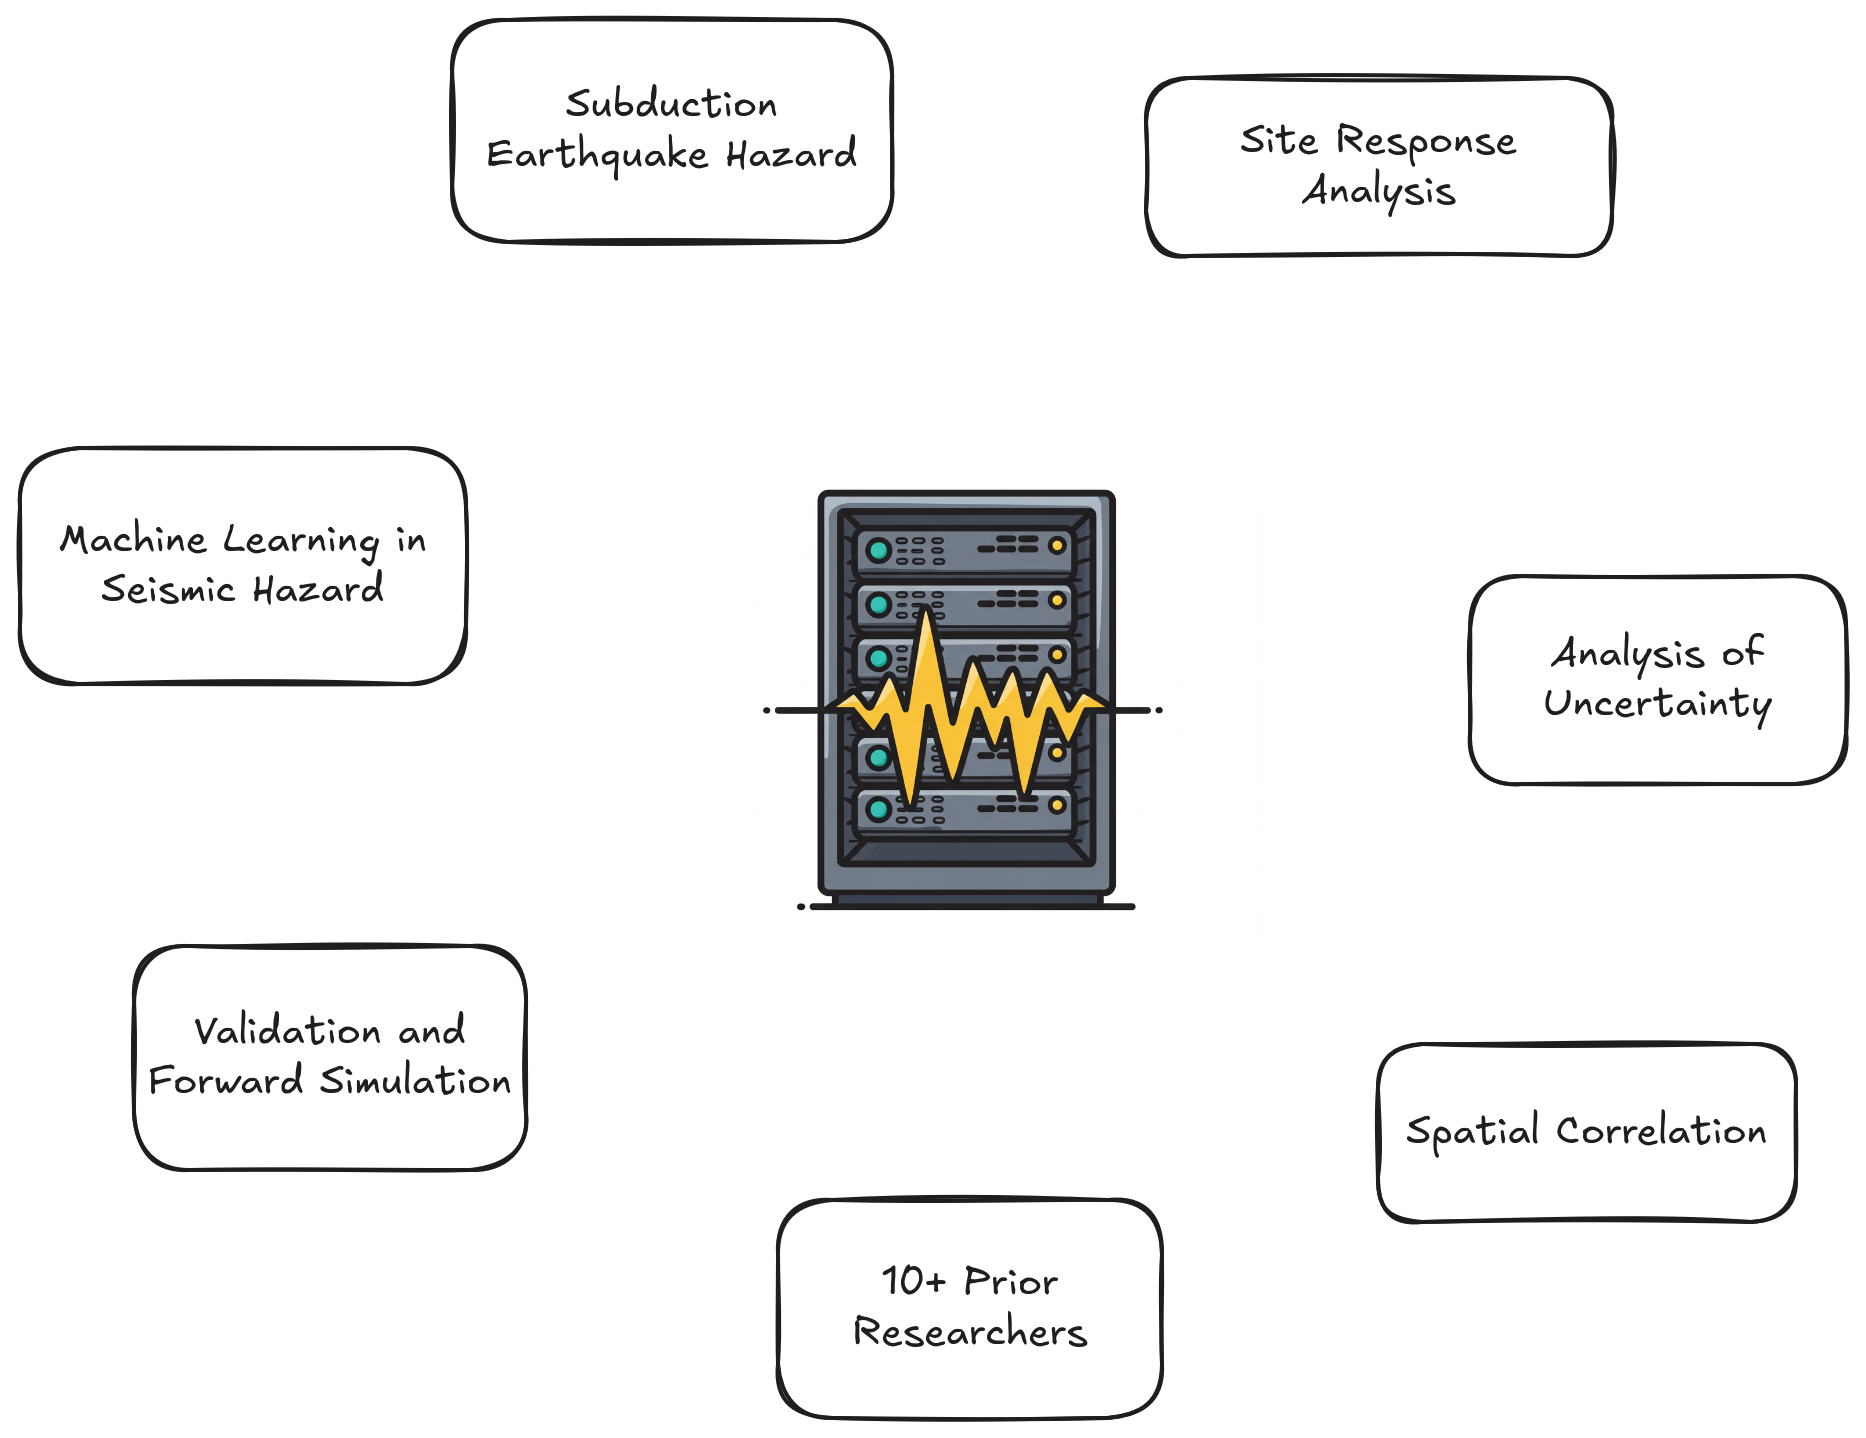
\includegraphics[width=.9\linewidth]{researcher.png}
\end{center}
\section*{The Old Simulation Stack}
\label{sec:orgf323305}
\subsection*{Basic Structure}
\label{sec:org8bfb187}
\begin{center}
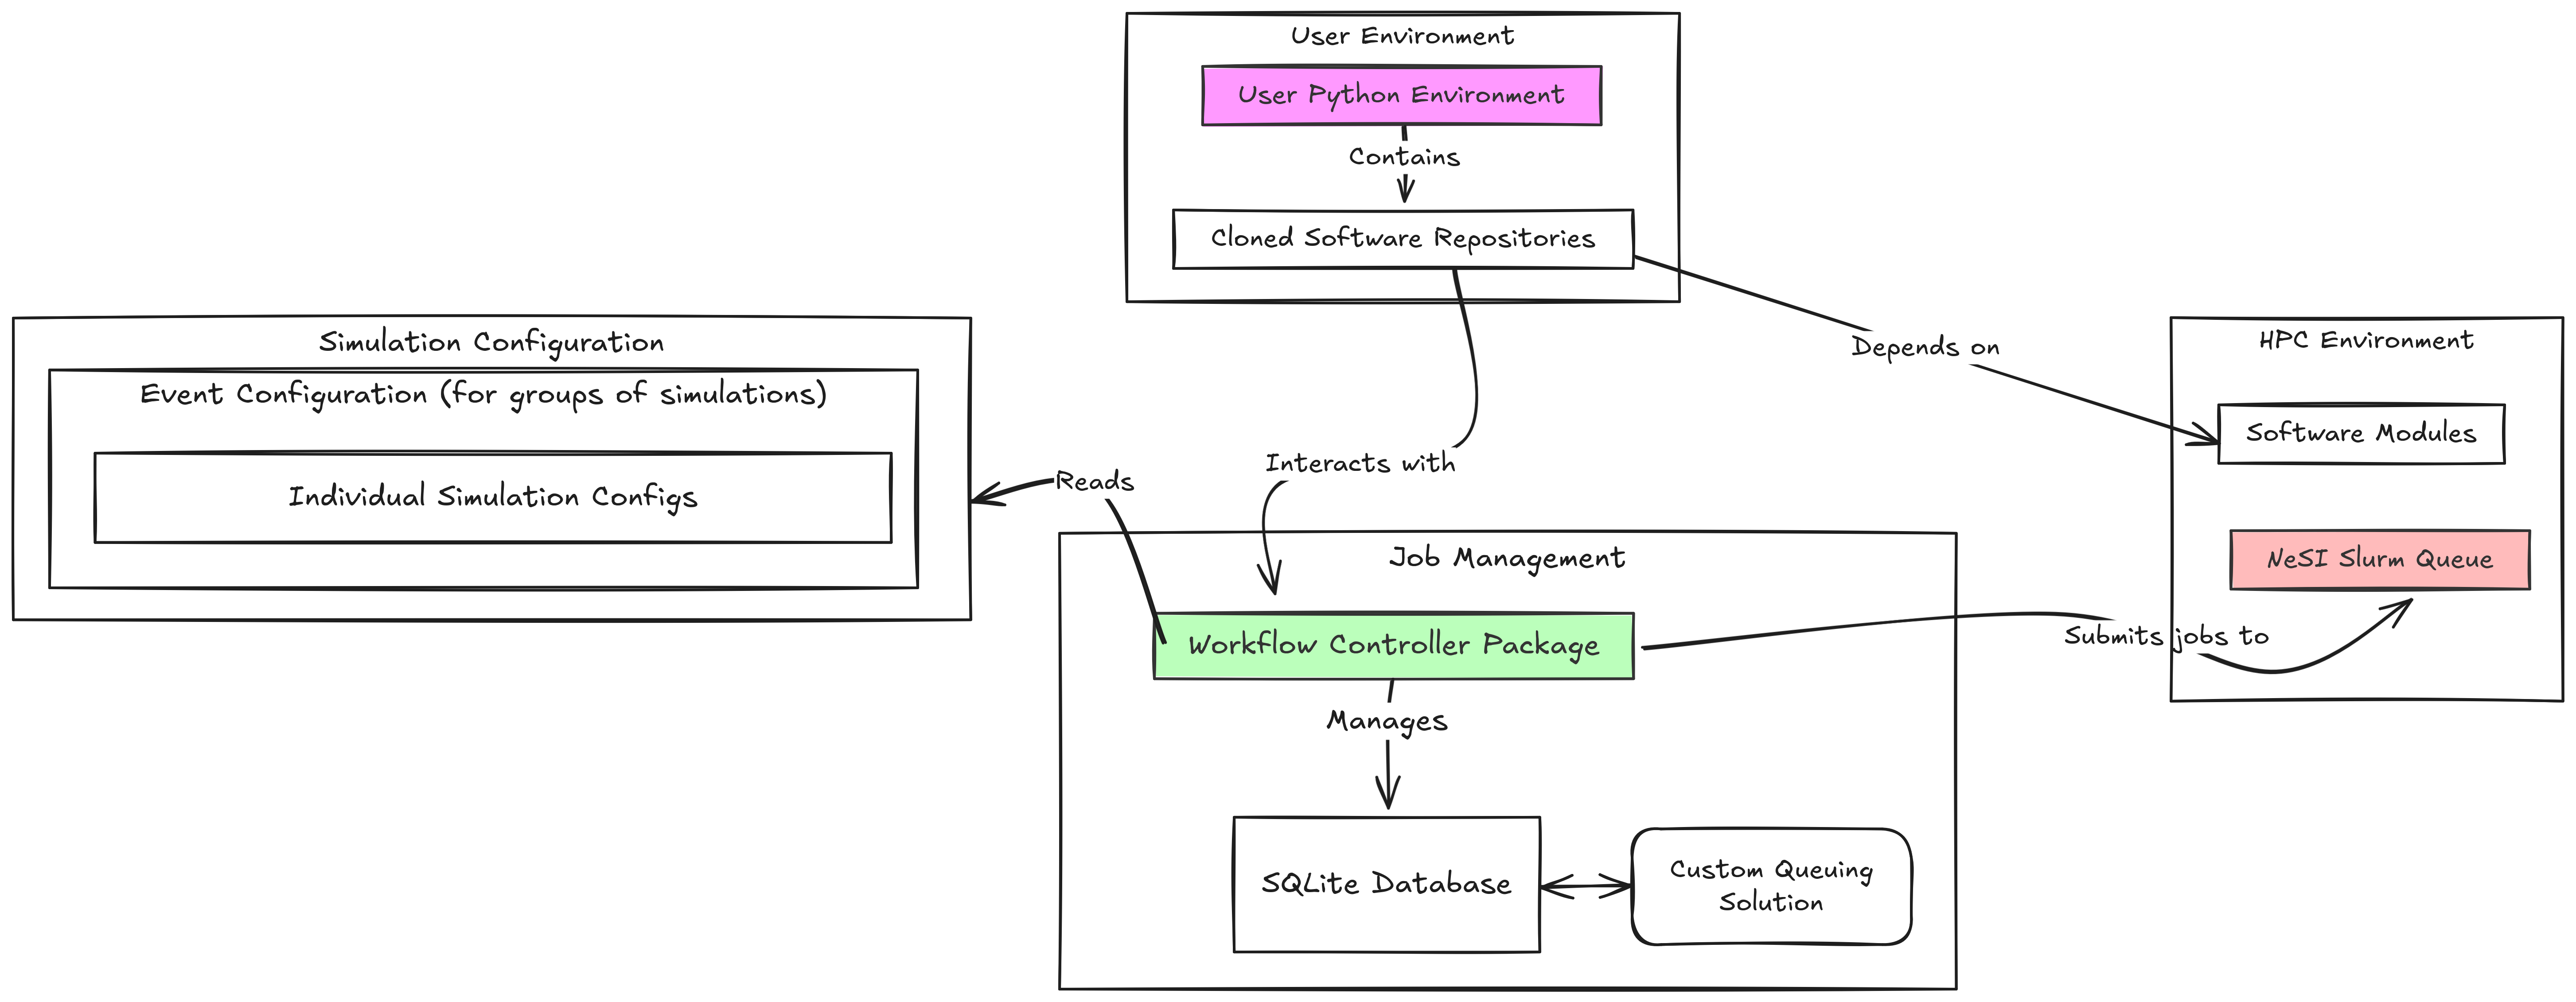
\includegraphics[width=.9\linewidth]{old_workflow.png}
\end{center}
\subsection*{The Problems}
\label{sec:org36e05d3}
\begin{itemize}
\item Cybershake-centric, unfriendly to researchers.
\item Entirely custom solutions for solved problems.
\item Complex, brittle, hard to reproduce.
\item \textbf{So much legacy code!}
\end{itemize}
\subsection*{Reproducing a Three-Year-Old Simulation}
\label{sec:org6abd72c}
\begin{enumerate}
\item Required our team lead one year,
\item Involved special tools to re-derive input values,
\item Ultimately impossible due to changing software.
\end{enumerate}
\begin{center}
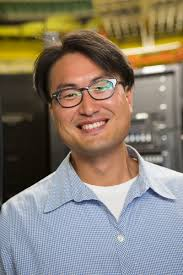
\includegraphics[width=.9\linewidth]{sung.jpg}
\end{center}
\section*{The New Workflow}
\label{sec:org6983df2}

\subsection*{Container + Workflow + Realisation = Simulation}
\label{sec:org6274222}
\begin{itemize}
\item \textbf{Container}: Reproducible software stack specification.
\item \textbf{Workflow}: Declarative software execution control.
\item \textbf{Realisation}: Declarative scientific parameter specification.
\end{itemize}
\subsection*{Containerisation}
\label{sec:orgdd131ca}
\begin{itemize}
\item Apptainer containers for software deployment.
\item All workflow stages within containers.
\item Archivable with future Cybershake versions.
\end{itemize}
\subsection*{Cylc Workflows}
\label{sec:org0eaa1b0}
\begin{itemize}
\item Developed at NIWA
\item Workflow stage composition with TOML-like syntax
\end{itemize}
\url{cylc.gif}
\subsection*{One-File Simulation Specification}
\label{sec:org35fd8f7}
\begin{center}
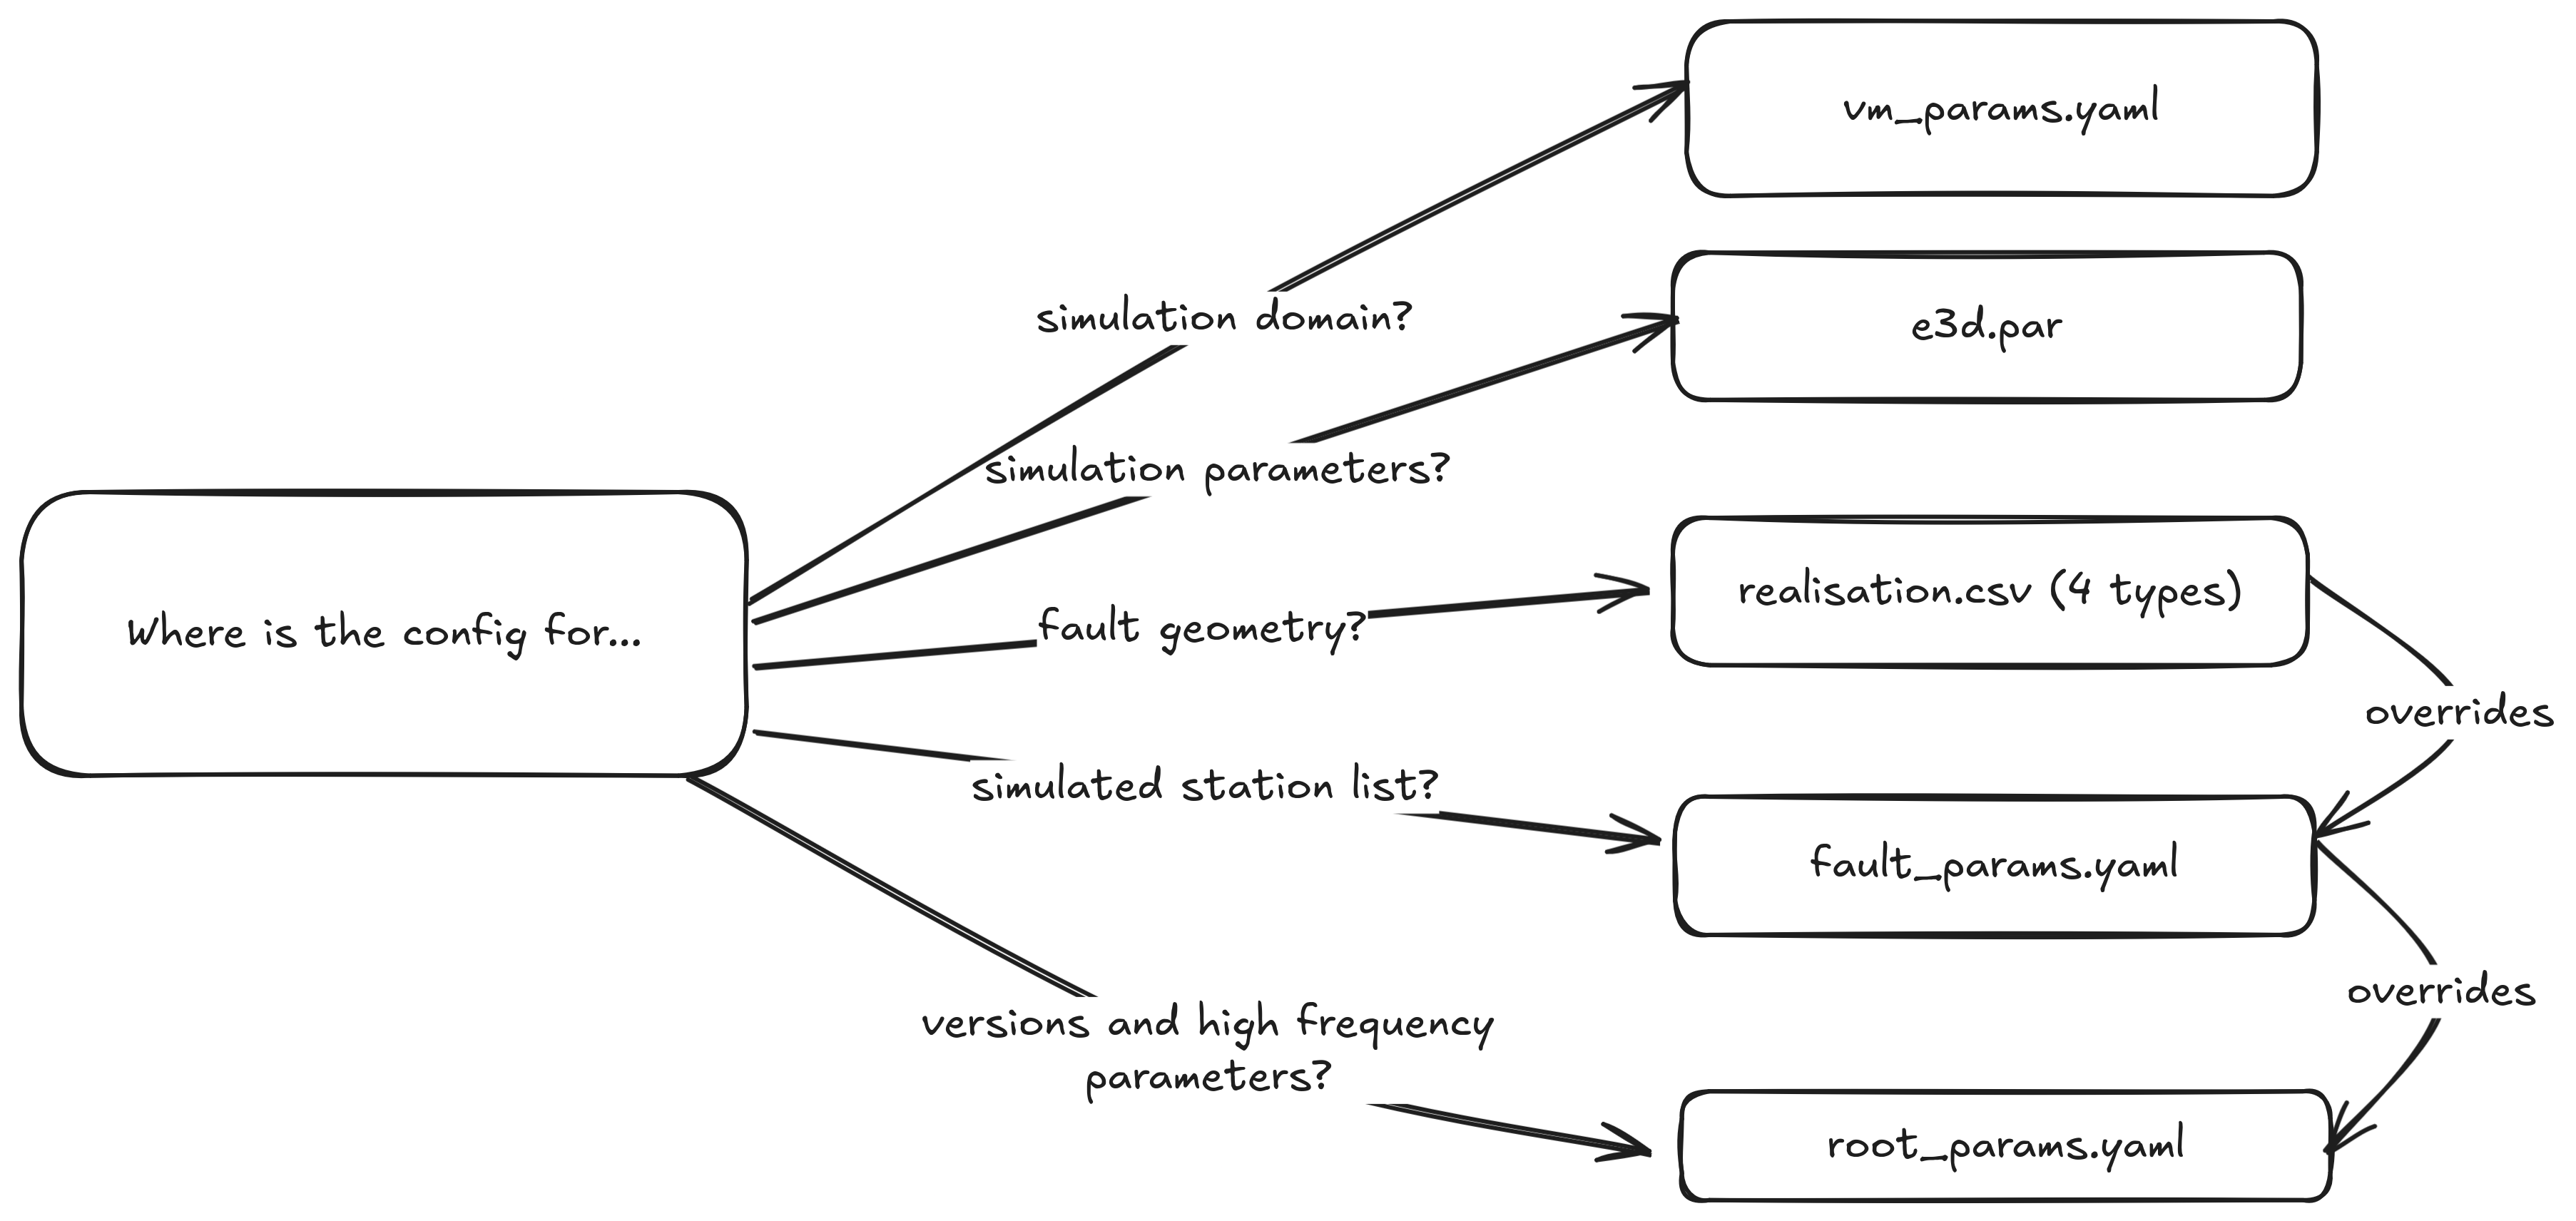
\includegraphics[width=.9\linewidth]{config.png}
\end{center}
\begin{verbatim}
realisation.json
      ┐
      ├── metadata
      │   ├── name: 3468575
      │   ├── version: 1
      │   ├── defaults_version: 24.2.2.2
      │   └── tag: gcmt
      ├── sources
      │   └── source_geometries [...]
      ├── rupture_propagation
      │   ├── rupture_causality_tree [...]
      │   ├── jump_points
      │   ├── rakes [...]
      │   ├── magnitudes [...]
      │   └── hypocentre [...]
      ├── srf
      │   ├── genslip_dt: 0.05
      │   ├── genslip_version: 5.4.2
      │   └── resolution: 0.2
      ├── seeds
      │   ├── nshm_to_realisation_seed: 554010839
      │   ├── rupture_propagation_seed: 1355831879
      │   ├── genslip_seed: 906043042
      [...]
\end{verbatim}
\subsection*{Workflow Planner}
\label{sec:org6e5d660}
\begin{itemize}
\item Workflow stages that compose together enables a flexible workflow planning tool.
\item Skip or set a goal for any stage to generate custom research workflows!
\end{itemize}
\begin{verbatim}
  $ plan-workflow 2024p910344 flow.cylc --source gcmt --goal im_calc \
      --excluding realisation_to_srf --archiving hf_sim
  You require the following files for your simulation:
  ┐
  └── cylc-src
      └── WORKFLOW_NAME
          └── input
              ├── 2024p910344
              │   ├── realisation.json
              │   │   └── srf: Configuration for SRF generation.
              │   └── realisation.srf: Contains the slip model for the realisation.
              ...
\end{verbatim}
\begin{center}
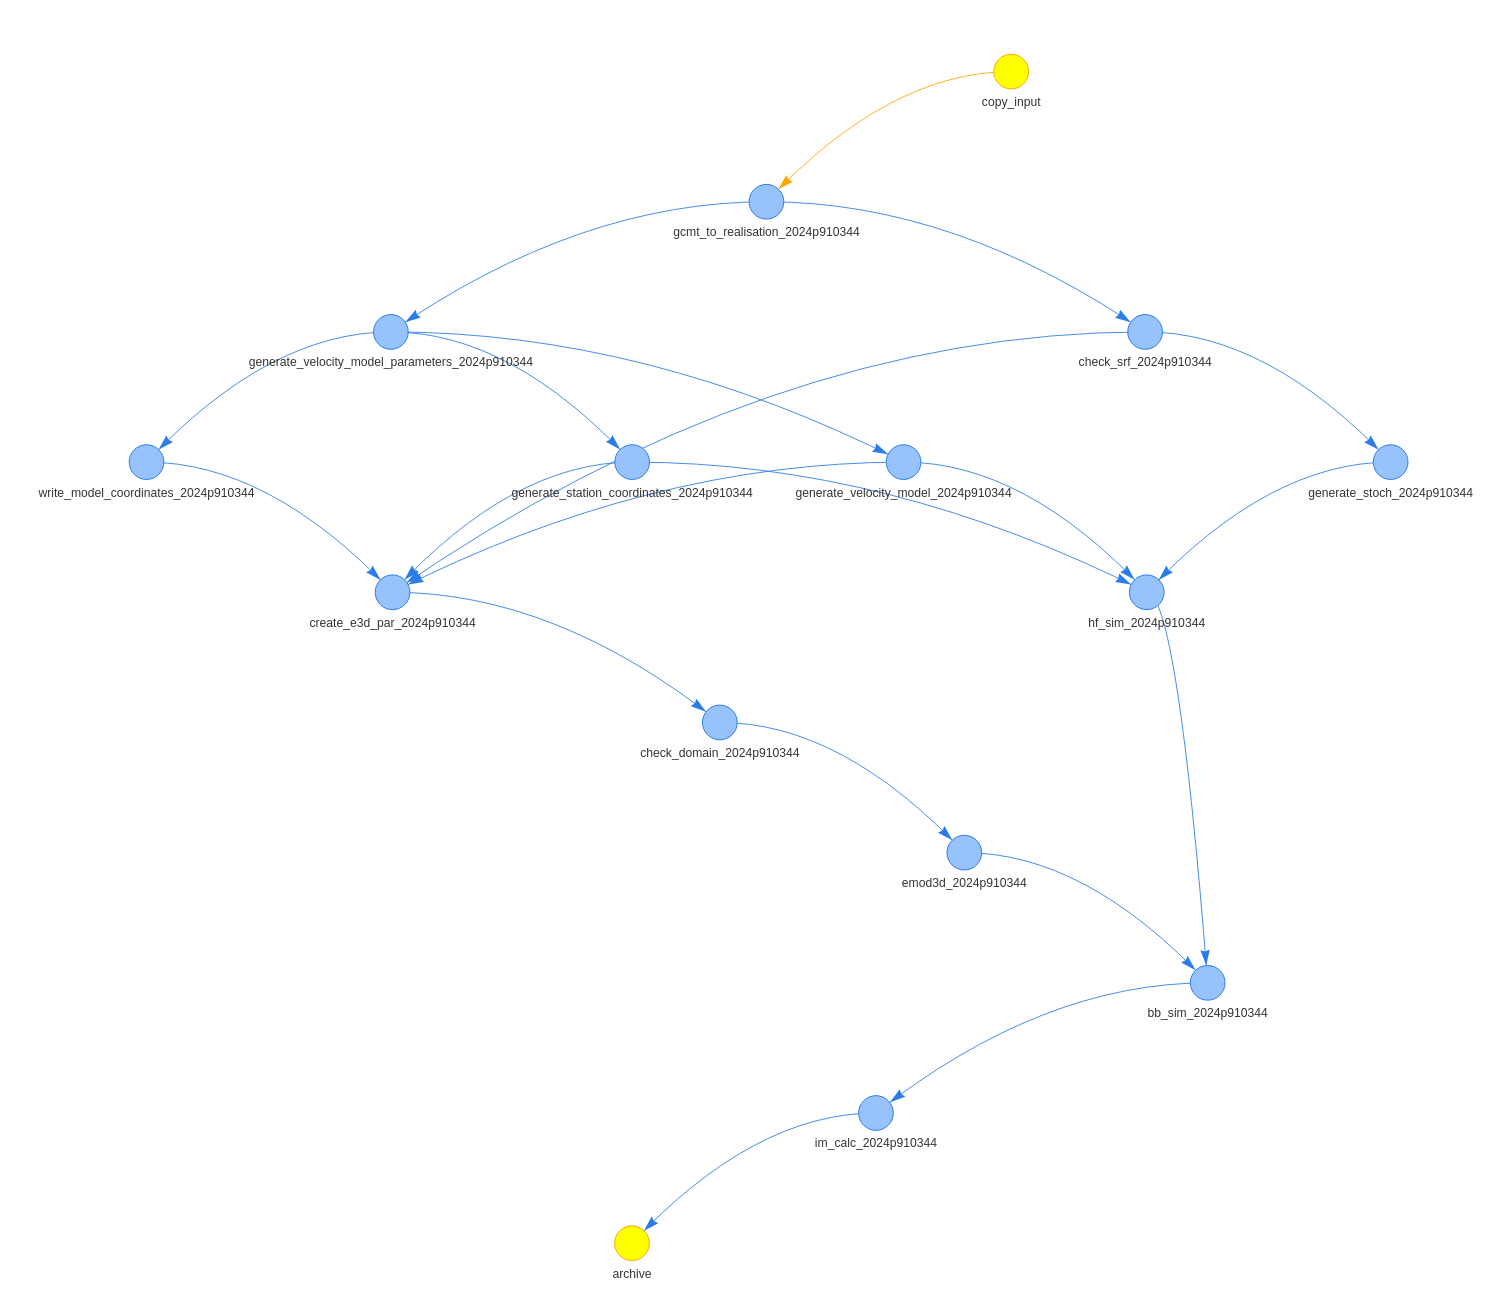
\includegraphics[width=.9\linewidth]{workflow_graph.png}
\end{center}
\subsection*{Hypothesis Testing}
\label{sec:org1441efc}

\begin{verbatim}
@given(st.integers(0, 50))
def test_prime_formula(n: int):
    """Test Euler's formula for primes."""
    assert is_prime(n**2 + n + 41)
\end{verbatim}
\begin{verbatim}
n = 40

    @given(st.integers(0, 50))
    def test_prime_formula(n: int):
>       assert is_prime(n**2 + n + 41)
E       assert False
\end{verbatim}
\begin{itemize}
\item Used to test thousands of examples for critical scientific code.
\item Potentially saves hundreds of thousands of wasted core-hours.
\end{itemize}
\section*{Key Takeaways}
\label{sec:org2d0d6e8}
\begin{itemize}
\item Make your workflows \textbf{declarative}.
\item Make your workflows \textbf{composable}.
\item Automate your testing.
\item Design for the \textbf{least-savvy user}.
\end{itemize}
\end{document}
